\documentclass[12pt,a4paper]{report}
\usepackage[bahasa]{babel}
\usepackage[utf8]{inputenc}
\usepackage[T1]{fontenc}
\usepackage{geometry}
\geometry{a4paper, margin=2.5cm, top=3cm, bottom=2.5cm, headheight=14.5pt}
\usepackage{xcolor}
\usepackage[most]{tcolorbox}
\usepackage{graphicx}
\usepackage{booktabs}
\usepackage{tabularx}
\usepackage{enumitem}
\usepackage[expansion=false]{microtype}
\usepackage{titlesec}
\usepackage{fancyhdr}
\usepackage{amsmath}
\usepackage{amssymb}

% Warna Korporat PLN (harus didefinisikan SEBELUM hypersetup)
\definecolor{plnblue}{RGB}{0,75,135}
\definecolor{plnorange}{RGB}{255,107,53}

\usepackage{hyperref}
\hypersetup{
    colorlinks=true,
    linkcolor=plnblue,
    urlcolor=plnblue,
    citecolor=plnblue
}

% Header & Footer
\pagestyle{fancy}
\fancyhf{}
\fancyhead[L]{\small\textbf{Modul 4.3: Bab 5 \& 6}}
\fancyhead[R]{\small Level 4 (Mastery) -- PLN}
\fancyfoot[C]{\small\thepage}
\renewcommand{\headrulewidth}{0.4pt}

% Format Heading
\titleformat{\chapter}[display]{\normalfont\huge\bfseries\color{plnblue}}{\chaptertitlename\ \thechapter}{20pt}{\Huge}
\titleformat{\section}{\Large\bfseries\color{plnblue}}{\thesection}{1em}{}
\titleformat{\subsection}{\large\bfseries\color{plnblue}}{\thesubsection}{1em}{}
\titlespacing*{\chapter}{0pt}{-30pt}{20pt}
\titlespacing*{\section}{0pt}{12pt}{8pt}
\titlespacing*{\subsection}{0pt}{10pt}{6pt}

% Custom Boxes
\newtcolorbox{plnbox}[1][]{%
  colback=plnblue!5!white, colframe=plnblue, fonttitle=\bfseries,
  title=#1, sharp corners, boxrule=0.8pt, breakable
}
\newtcolorbox{warnbox}{%
  colback=plnorange!10, colframe=plnorange, fonttitle=\bfseries,
  title=Catatan Batasan Materi, sharp corners, breakable
}
\newtcolorbox{outputbox}{%
  colback=green!10, colframe=green!50!black, fonttitle=\bfseries,
  title=Output Wajib, sharp corners, breakable
}

% List styling
\setlist[itemize]{leftmargin=*, topsep=2pt, itemsep=2pt}
\setlist[enumerate]{leftmargin=*, topsep=2pt, itemsep=2pt}

\begin{document}

% ================= COVER STANDALONE =================
\begin{titlepage}
\centering
\vspace*{1.5cm}
{\Huge\bfseries\color{plnblue} MODUL 4.3 (Penutup)}\\[0.4cm]
{\LARGE\bfseries Bab 5 \& 6: Penghitungan Efisiensi, ROI, \& Penutup}\\[0.8cm]
\rule{0.8\linewidth}{0.6pt}\\[0.6cm]
{\large Program Penguatan Kompetensi Tata Kelola Kearsipan}\\
{\large Level 4 (Mastery)}\\[1.2cm]
{\large Disusun Khusus untuk: \textbf{PT PLN (Persero)}}\\
{\large Target Peserta: Manajemen Atas (MA)}\\[2.5cm]
\includegraphics[width=4cm]{example-image}
\vfill
{\small Dokumen ini dapat dikompilasi secara terpisah dari Bab 1--4}
\end{titlepage}

\newpage
% ================= BAB 5 =================
\setcounter{chapter}{4}
\chapter{Penghitungan Efisiensi \& ROI}
\textit{Durasi Fasilitasi: 15 Menit} \quad \textit{Kriteria Penilaian: 4.3.4}

\section{Metodologi Pengukuran Kinerja Kearsipan}

Bagi jajaran Manajemen Atas, tata kelola kearsipan tidak boleh lagi dipandang sebagai pusat biaya (\textit{cost center}) yang kinerjanya semata-mata diukur dari volume dokumen yang digudangkan. Di era ekosistem kelistrikan terintegrasi, unit kearsipan harus bertransformasi menjadi pusat penciptaan nilai (\textit{value center}). Oleh karena itu, efektivitas dari inisiatif optimalisasi prosedur tidak diukur dari tingginya anggaran IT atau kerumitan teknologi yang dibeli, melainkan dari \textbf{perubahan nyata pada efisiensi proses bisnis dan mitigasi risiko kepatuhan}.

Dalam konteks ini, \textbf{mitigasi risiko kepatuhan} (atau mitigasi risiko bisnis) adalah langkah evaluasi secara kualitatif dan kuantitatif untuk menekan potensi ancaman kerugian operasional dan finansial akibat ketidakpatuhan terhadap regulasi kearsipan.

Metodologi pengukuran kinerja kearsipan dalam modul ini secara khusus dirancang untuk menjembatani kesenjangan antara teori kearsipan dengan bahasa bisnis BUMN. Metodologi ini bertumpu pada kemampuan mengkuantifikasi kemacetan operasional menjadi nominal kerugian, dan sebaliknya, menerjemahkan kelancaran alur persetujuan menjadi \textit{Return on Investment} (ROI) yang dapat diaudit. Dengan pendekatan ini, setiap rencana optimalisasi prosedur memiliki basis argumen yang rasional sebelum diusulkan ke komite investasi.

\begin{figure}[htbp]
\centering
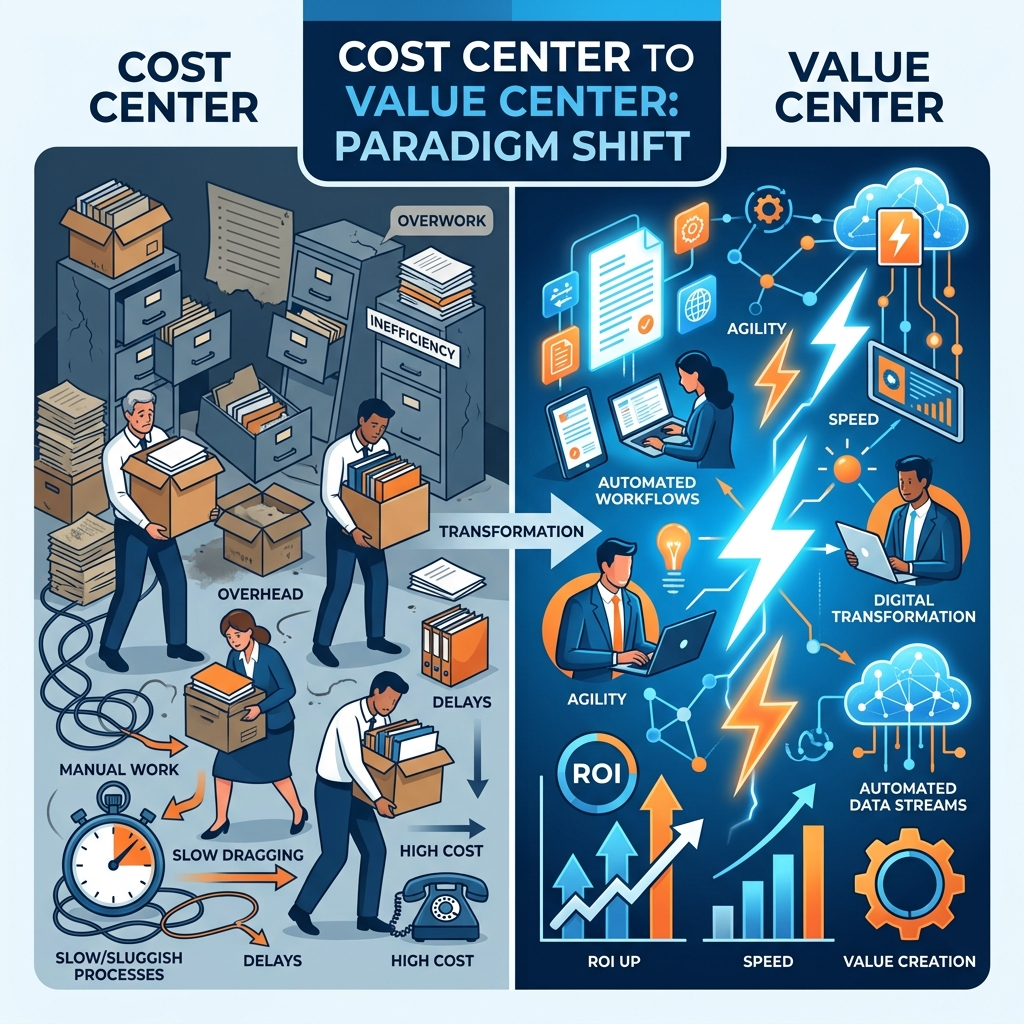
\includegraphics[width=0.9\textwidth]{infografis_paradigma.png}
\caption{Visualisasi Pergeseran Paradigma Kearsipan: Dari \textit{Cost Center} Menuju \textit{Value Center}}
\label{fig:paradigma}
\end{figure}

\subsection{Indikator Kinerja Utama (KPI)}
Dalam perbaikan tata kelola, \textbf{intervensi operasional} (atau optimalisasi) merujuk pada langkah-langkah atau inisiatif perbaikan spesifik yang diterapkan secara langsung pada prosedur yang sudah ada guna "mengobati" inefisiensi---seperti proses manual yang lambat atau rentan kesalahan---menjadi cara kerja baru yang terintegrasi. Secara singkat, \textit{jika analisis ROI adalah cara mengukur keuntungannya, maka intervensi operasional adalah tindakan perbaikan (solusi teknis dan prosedural) yang dieksekusi di lapangan untuk mendapatkan keuntungan tersebut}.

Untuk mengetahui apakah sebuah intervensi operasional berhasil atau tidak, dampaknya wajib diukur menggunakan metrik spesifik yang dapat dilacak kemajuannya. Tidak semua metrik relevan untuk Manajemen Atas. Oleh sebab itu, \textbf{Tabel 5.1} menyajikan empat indikator kunci terbaik yang berfokus pada waktu siklus (\textit{Cycle Time}), ketepatan awal (\textit{First-Time Accuracy}), waktu temu kembali (\textit{Retrieval Speed}), dan tingkat kepatuhan prosedur (\textit{Compliance Rate}). Pemantauan keempat indikator ini akan langsung menyoroti seberapa sehat tata kelola kearsipan berjalan di suatu unit.

\vspace{0.3cm}
\noindent
{\small\bfseries Tabel 5.1: Indikator Kinerja Proses Kearsipan Terintegrasi}

\vspace{0.2cm}
\noindent
\small
\begin{tabularx}{\textwidth}{@{} >{\raggedright\arraybackslash}X >{\raggedright\arraybackslash}X >{\raggedright\arraybackslash}X @{}}
\toprule
\textbf{Indikator} & \textbf{Definisi Operasional} & \textbf{Target Realistis (Setelah Optimalisasi)} \\
\midrule
\textbf{Waktu Siklus} & Waktu total dari penciptaan/transaksi hingga arsip tervalidasi \& tersimpan & $\downarrow$ 40--60\% (misal: 5 hari $\rightarrow$ 1--2 hari) \\
\textbf{Ketepatan Awal} & Persentase arsip yang lolos validasi metadata tanpa revisi & $\uparrow$ $\geq$90\% \\
\textbf{Waktu Temu Kembali} & Waktu temu kembali arsip berdasarkan query bisnis/audit & $\downarrow$ $<$30 detik (digital) \\
\textbf{Tingkat Kepatuhan Prosedur} & Persentase proses yang memenuhi SLA, retensi, \& jejak audit & $\uparrow$ $\geq$95\% \\
\bottomrule
\end{tabularx}
\vspace{0.3cm}

Secara operasional, untuk mendapatkan pengukuran yang valid pada indikator \textbf{Waktu Siklus (\textit{Cycle Time})}, penghitungan durasi tidak boleh berhenti dan dianggap selesai hanya pada saat draf pelaporan atau dokumen telah diketik. Sistem informasi atau pengelola proses harus dengan disiplin mencatat dua titik waktu utama:
\begin{enumerate}[leftmargin=*]
    \item \textbf{Titik Awal (\textit{Start Time}):} Waktu \textit{timestamp} sistematis saat dokumen atau transaksi pertama kali diciptakan (misalnya detik saat draf mulai di-\textit{generate} di portal operasional).
    \item \textbf{Titik Akhir (\textit{End Time}):} Waktu \textit{timestamp} sistematis saat dokumen tersebut telah 100\% selesai melewati alur persetujuan, metadatanya divalidasi, dan secara resmi \textit{tersimpan} ke dalam repositori kearsipan digital perwakilan fungsional.
\end{enumerate}

Sementara itu, untuk indikator \textbf{Ketepatan Awal (\textit{First-Time Accuracy})}, langkah pengukuran cukup memonitor persentase \textbf{jumlah dokumen yang berhasil tervalidasi dengan benar di percobaan pertama berbanding total volume dokumen yang masuk}. Sebagai ilutrasi dari studi kasus penciptaan dokumen:
\begin{itemize}[leftmargin=*]
    \item Jika dari total volume \textbf{1.200 arsip} per tahun, diketahui terdapat \textbf{420 arsip} yang gagal validasi sehingga harus direvisi akibat \textit{error input} manual.
    \item Angka ini berarti tingkat kesalahan mencetak persentase 35\%, sehingga kinerja \textit{First-Time Accuracy} unit tersebut tercatat hanya sebesar \textbf{65\%}.
    \item Pasca-optimalisasi, laju dokumen yang sukses lolos tanpa revisi tersebut dapat melonjak naik hingga misalnya \textbf{96\%}, yang mana secara meyakinkan melampaui standar wajib minimum $\geq$90\%.
\end{itemize}

Terakhir, untuk indikator \textbf{Waktu Temu Kembali (\textit{Retrieval Speed})}, metode pengukurannya bergantung secara spesifik pada ekosistem penyimpanan itu sendiri:
\begin{itemize}[leftmargin=*]
    \item \textbf{Di lingkungan arsip fisik:} Waktu dihitung dari mulai staf menerima \textit{request} pencarian hingga menemukan kertasnya di gudang letak \textit{filing cabinet}.
    \item \textbf{Di lingkungan arsip digital:} Waktu dihitung berdasarkan kecepatan sistem komputer dalam menampilkan dokumen (\textit{query speed}) dan akurasi hasil navigasi dari \textit{search engine} kearsipan.
\end{itemize}

Terakhir, untuk indikator \textbf{Tingkat Kepatuhan Prosedur (\textit{Compliance Rate})}, pengukuran tidak boleh hanya melihat apakah dokumen "sudah ada di sistem", melainkan harus memastikan apakah dokumen tersebut memenuhi standar kriteria validitas serta \textbf{Imunitas Hukum (\textit{Legal Admissibility})} sebagai berikut:
\begin{itemize}[leftmargin=*]
    \item \textbf{Kesatuan Isi, Struktur, dan Konteks (Kelengkapan Jejak Audit):} Arsip harus memiliki kronologi (\textit{audit trail log}) yang utuh. Tanpa ini, dokumen tersebut hanyalah \textit{file} yatim piatu yang cacat hukum.
    \item \textbf{Disahkan dengan Tanda Tangan Elektronik (TTE) Tersertifikasi:} Sesuai PP 71/2019, otorisasi wajib menggunakan TTE Tersertifikasi untuk memberikan kekuatan hukum yang sah dan mutlak.
    \item \textbf{Bersifat \textit{Immutable} (Terkunci dan Tidak Dapat Direkayasa):} Dokumen dan metadata harus direkatkan oleh algoritma kriptografi (\textit{Hash Integrity}) sehingga tidak dapat diubah lagi keutuhannya sejak detik disetujui.
    \item \textbf{Kelengkapan 12 Metadata Wajib Otomatis:} Menjamin 12 \textit{field} metadata (ID, Timestamp, Hash, dll.) ditarik secara otomatis oleh mesin guna membatasi celah \textit{human error}.
    \item \textbf{Tercipta dari Sumber Kebenaran Tunggal (\textit{Single Source of Truth}):} Data mengalir otonom dari sistem sumber transaksi (ERP/Sistem Operasional) ke repositori tanpa penginputan ulang manual.
\end{itemize}

Sedangkan untuk dokumen yang diciptakan dalam bentuk fisik (\textbf{Arsip Hibrida}), kriteria kepatuhannya diukur berdasarkan:
\begin{itemize}[leftmargin=*]
    \item \textbf{Sinkronisasi Lokasi Fisik \& Digital (\textit{Finding Aid Consistency}):} Kepatuhan diukur dari apakah lokasi fisik dokumen (Gedung, Ruang, Rak, Boks, hingga Folder) sudah tercatat secara presisi di database sistem kearsipan sesaat setelah dokumen tercipta. Tanpa sinkronisasi ini, dokumen fisik dianggap tidak patuh karena tidak dapat ditemukan kembali dalam SLA yang ditentukan.
    \item \textbf{Otentisitas Otoritas Basah \& Cap Unit:} Meskipun fisik, dokumen harus memenuhi unsur keabsahan tradisional: tanda tangan basah pejabat berwenang dan stempel unit asli. Kepatuhan prosedur mewajibkan adanya verifikasi visual atas kelengkapan "atribut sah" ini sebelum dokumen masuk ke tahap penyimpanan.
    \item \textbf{Keberadaan Metadata Penanda (\textit{Proxy Metadata}):} Dokumen fisik wajib memiliki "kembaran digital" berupa lembar metadata di sistem yang mencatat minimal: Tanggal Cipta, Nomor Dokumen, dan Ringkasan Isi. Kriteria patuh terpenuhi jika petugas tidak perlu lagi membaca isi dokumen fisik hanya untuk mengetahui apa isinya.
    \item \textbf{Kepatuhan Pelabelan Retensi (\textit{Physical Retention Labeling}):} Setiap boks atau folder fisik harus memiliki label retensi yang selaras dengan database JRA (Jadwal Retensi Arsip). Prosedur dianggap patuh jika tanggal pemusnahan/pemindahan yang tertera pada boks fisik sama persis dengan yang tercatat di sistem digital.
    \item \textbf{Integritas Log Mutasi Fisik:} Setiap perpindahan dokumen fisik (dari meja kerja ke rak aktif, atau dipinjam unit lain) wajib terekam dalam log mutasi. Kepatuhan prosedur diukur dari kesesuaian antara "posisi riil" dokumen di gudang dengan "status posisi" dokumen di sistem.
\end{itemize}
\begin{plnbox}[Kacamata Arsiparis: Keseimbangan Kecepatan \& Integritas]
\small
Dalam mengevaluasi KPI tersebut, Manajemen Atas perlu mewaspadai satu jebakan umum (\textit{logical fallacy}) dalam otomatisasi: \textbf{berasumsi bahwa kecepatan identik dengan kualitas tata kelola}. 

\begin{itemize}[leftmargin=*]
    \item \textbf{Imunitas Hukum (\textit{Legal Admissibility}):} KPI ketepatan awal bukan sekadar mencegah staf mengulang pekerjaan. Keakuratan metadata otomatis dan keutuhan \textit{hash integrity} adalah bukti primer berkekuatan hukum jika PLN diaudit BPK atau menghadapi litigasi.
    \item \textbf{ROI dari Pemusnahan Data (\textit{Disposition}):} Perhatian tata kelola siklus hidup arsip secara utuh tidak boleh berhenti hanya pada fase penciptaan. Penahanan \textit{junk data} atau dokumen digital kadaluwarsa melewati masa Jadwal Retensi Arsip (JRA) demi alasan "berjaga-jaga" justru membebani biaya \textit{server} dan memicu risiko audit (\textit{e-discovery risk}). Tata kelola sejati mensyaratkan otomasi pemusnahan yang legal.
\end{itemize}
\end{plnbox}

\begin{warnbox}
\textbf{Catatan Batasan Materi:} Pengukuran ini berfokus pada \textbf{efektivitas alur kerja dan kepatuhan proses}, bukan pada \textit{uptime server}, \textit{throughput database}, atau \textit{kapasitas penyimpanan teknis} yang merupakan domain evaluasi infrastruktur (Modul 4.1/4.2).
\end{warnbox}

\subsection{Metode Penghitungan Efisiensi \& ROI}
Untuk meyakinkan pemangku kepentingan, potensi peningkatan efektivitas dari keempat indikator di atas harus dikuantifikasi secara sederhana namun dapat diaudit. Gunakan pendekatan \textbf{Time-Cost-Risk Saving}:

\begin{enumerate}[leftmargin=*]
    \item \textbf{Penghematan Waktu $\times$ Biaya:} 
    \begin{multline*}
    \text{ROI Waktu} = (\text{Waktu Siklus Lama} - \text{Waktu Siklus Baru}) \\
    \times\; \text{Volume Proses/Tahun} \times \text{Biaya Rata-Rata/Jam}
    \end{multline*}
    \item \textbf{Reduksi Biaya Kesalahan:} Hitung potensi penghematan dari penurunan revisi, pencetakan ulang, denda keterlambatan pelaporan, atau biaya audit temuan.
    \item \textbf{Mitigasi Risiko Kepatuhan (atau Risiko Bisnis):} Nilai kualitatif-kuantitatif dari penurunan risiko kehilangan arsip vital, pelanggaran PP 71/2019, atau temuan audit BPK.
\end{enumerate}

\begin{plnbox}[PLN Context Box]
\textbf{Ilustrasi Kalkulasi Sederhana (Proses arsip perintah kerja (SPK) Pemeliharaan GI):}
\begin{itemize}[nosep]
    \item Volume: 1.200 arsip perintah kerja (SPK)/tahun
    \item Waktu siklus: 5 hari $\rightarrow$ 1 hari (hemat 4 hari/arsip perintah kerja (SPK))
    \item Biaya tenaga kerja \& overhead: Rp 150.000/hari
    \item \textbf{Penghematan Waktu} = $1.200 \times 4 \times 150.000 = \textbf{Rp 720.000.000/tahun}$
    \item \textbf{Dampak Tambahan:} Error metadata $\downarrow$ 85\%, temuan audit administratif $\rightarrow$ 0
\end{itemize}
\end{plnbox}

\section{Studi Kasus End-to-End: Transformasi arsip perintah kerja (SPK) Pemeliharaan GI 150 kV}
\label{sec:studikasus}

Studi kasus berikut menyajikan simulasi lengkap penerapan optimalisasi alur kerja kearsipan pada proses Work Order (arsip perintah kerja (SPK)) pemeliharaan Gardu Induk 150 kV, dari kondisi awal hingga hasil implementasi pilot selama 90 hari.

\subsubsection*{A. Profil Unit \& Konteks}
\begin{itemize}[nosep, leftmargin=*]
    \item \textbf{Unit:} UIT Jawa Bagian Tengah -- Area Pemeliharaan Gardu Induk
    \item \textbf{Cakupan:} 48 Gardu Induk 150 kV, 12 tim teknisi pemeliharaan
    \item \textbf{Volume:} $\pm$1.200 Work Order pemeliharaan/tahun (rata-rata 100 arsip perintah kerja (SPK)/bulan)
    \item \textbf{Sistem Yang Ada:} Sistem Operasional (input arsip perintah kerja (SPK)), Filing cabinet \& folder bersama (arsip), Email (alur persetujuan)
\end{itemize}

\subsubsection*{B. Kondisi Sebelum Optimalisasi (As-Is)}

\vspace{0.3cm}
\noindent
{\small\bfseries Tabel: Analisis Kondisi As-Is -- Dampak Proses Manual}

\vspace{0.2cm}
\noindent
\small
\begin{tabularx}{\textwidth}{@{} >{\raggedright\arraybackslash}X >{\raggedright\arraybackslash}X r @{}}
\toprule
\textbf{Masalah} & \textbf{Dampak Operasional} & \textbf{Kerugian/Tahun} \\
\midrule
Waktu siklus rata-rata 5 hari/arsip perintah kerja (SPK) & Penundaan pelaporan kesiapan aset ke Dispatcher & Rp 720.000.000 \\
Error metadata 35\% (input manual) & 420 arsip perintah kerja (SPK)/tahun perlu revisi, rata-rata 2 jam/revisi & Rp 52.500.000 \\
Kehilangan 8 dokumen arsip/tahun & Temuan audit BPK, potensi sanksi administratif & Rp 200.000.000 \\
Waktu temu kembali 15--30 menit & Keterlambatan respons saat audit mendadak & Rp 37.500.000 \\
\addlinespace
\multicolumn{2}{@{}l}{\textbf{Total Estimasi Kerugian Tahunan}} & \textbf{Rp 1.010.000.000} \\
\bottomrule
\end{tabularx}

\begin{plnbox}[Catatan Perhitungan]
\small
\begin{itemize}[nosep, leftmargin=*]
    \item Biaya waktu siklus: 1.200 arsip perintah kerja (SPK) $\times$ 4 hari terbuang $\times$ Rp 150.000/hari = Rp 720 juta
    \item Biaya revisi: 420 arsip perintah kerja (SPK) $\times$ 2 jam $\times$ Rp 62.500/jam = Rp 52,5 juta
    \item Biaya kehilangan arsip: 8 kasus $\times$ Rp 25 juta (biaya rekonstruksi + risiko sanksi) = Rp 200 juta
    \item Biaya waktu temu kembali yang lambat: 1.200 arsip perintah kerja (SPK) $\times$ 0,25 jam terbuang $\times$ Rp 125.000/jam = Rp 37,5 juta
\end{itemize}
\end{plnbox}

\subsubsection*{C. Intervensi Optimalisasi yang Diterapkan}

\begin{enumerate}[leftmargin=*, nosep]
    \item \textbf{Pemicu Otomatis:} Status \textit{Selesai} di Sistem Operasional memicu auto-generate draft arsip arsip perintah kerja (SPK) + 12 field metadata wajib (ID GI, tanggal, teknisi, sparepart, kategori pemeliharaan, dll.)
    \item \textbf{Validasi Digital:} Supervisor melakukan validasi via Sistem Tata Persuratan Digital dengan SLA maksimal 1$\times$24 jam kerja; eskalasi otomatis ke Manajer Area jika terlampaui
    \item \textbf{Penyimpanan Langsung:} Arsip tervalidasi langsung tersimpan di repositori digital dengan hash integrity \& audit trail immutable
    \item \textbf{SOP Digital 7 Komponen:} Prosedur baku mencakup trigger, metadata, SLA, exception handling, dan referensi regulasi
\end{enumerate}

\subsubsection*{D. Hasil Setelah 90 Hari Pilot (To-Be)}

\vspace{0.3cm}
\noindent
{\small\bfseries Tabel: Perbandingan KPI -- Sebelum vs Sesudah Optimalisasi}

\vspace{0.2cm}
\noindent
\small
\begin{tabularx}{\textwidth}{@{} >{\raggedright\arraybackslash}X c c c @{}}
\toprule
\textbf{Indikator Kinerja} & \textbf{Sebelum} & \textbf{Sesudah} & \textbf{Peningkatan} \\
\midrule
Waktu Siklus (rata-rata) & 5 hari & 0,8 hari & $\downarrow$ 84\% \\
Ketepatan Awal & 65\% & 96\% & $\uparrow$ 31 poin \\
Waktu Temu Kembali & 15--30 menit & $<$20 detik & $\downarrow$ 99\% \\
Tingkat Kepatuhan Prosedur & 72\% & 98\% & $\uparrow$ 26 poin \\
Kehilangan Arsip & 8 kasus/tahun & 0 kasus & $\downarrow$ 100\% \\
Temuan Audit BPK & 3 temuan/tahun & 0 temuan & $\downarrow$ 100\% \\
\bottomrule
\end{tabularx}

\subsubsection*{E. Kalkulasi ROI \& Dampak Finansial}

\vspace{0.3cm}
\noindent
{\small\bfseries Tabel: Ringkasan ROI Transformasi Kearsipan GI 150 kV}

\vspace{0.2cm}
\noindent
\small
\begin{tabularx}{\textwidth}{@{} >{\raggedright\arraybackslash}X r @{}}
\toprule
\textbf{Komponen} & \textbf{Nilai (Rp/tahun)} \\
\midrule
\multicolumn{2}{@{}l}{\textbf{\color{plnblue}Penghematan (Benefit)}} \\
\quad Penghematan waktu siklus (1.200 arsip perintah kerja (SPK) $\times$ 4,2 hari $\times$ Rp 150.000) & 756.000.000 \\
\quad Reduksi biaya revisi metadata ($\downarrow$ 85\%) & 44.625.000 \\
\quad Eliminasi risiko kehilangan arsip & 200.000.000 \\
\quad Efisiensi waktu temu kembali & 36.000.000 \\
\addlinespace
\textbf{Total Benefit Tahunan} & \textbf{1.036.625.000} \\
\addlinespace
\multicolumn{2}{@{}l}{\textbf{\color{red}Biaya Implementasi (Cost) -- Tahun Pertama}} \\
\quad Konfigurasi pemicu otomatis \& template SOP & 75.000.000 \\
\quad Pelatihan 48 personel (3 batch) & 36.000.000 \\
\quad Pendampingan konsultan (90 hari pilot) & 50.000.000 \\
\addlinespace
\textbf{Total Cost Tahun Pertama} & \textbf{161.000.000} \\
\midrule
\textbf{Net Benefit Tahun Pertama} & \textbf{875.625.000} \\
\textbf{ROI Tahun Pertama} & \textbf{544\%} \\
\textbf{Payback Period} & \textbf{$<$ 2 bulan} \\
\bottomrule
\end{tabularx}

\subsubsection*{F. Lessons Learned}
\begin{enumerate}[leftmargin=*, nosep]
    \item \textbf{Quick Win Paling Berdampak:} Eliminasi langkah cetak-scan-upload memberikan penghematan waktu terbesar (60\% dari total penghematan waktu siklus) untuk dokumen rutin. Untuk dokumen legal/kontrak yang wajib dipertahankan fisiknya secara hibrida, penghematan didapat dari otomasi \textit{metadata tracking}-nya.
    \item \textbf{Faktor Keberhasilan Kritis:} Dukungan aktif Manajer Area sebagai champion proyek dan penegakan SLA validasi 1$\times$24 jam tanpa pengecualian.
    \item \textbf{Hambatan yang Ditemui:} Resistensi awal dari 3 supervisor senior yang terbiasa tanda tangan basah -- diatasi dengan pendampingan 1-on-1 dan demonstrasi jejak audit digital yang lebih kuat secara hukum.
    \item \textbf{Rekomendasi Skalabilitas:} Hasil pilot layak direplikasi ke seluruh UIT dengan penyesuaian minor pada template metadata sesuai karakteristik aset masing-masing area.
\end{enumerate}

\begin{outputbox}
\textbf{Nilai Strategis Studi Kasus:} Dengan investasi Rp 161 juta, unit ini menghemat lebih dari \textbf{Rp 1 miliar/tahun} dan mengeliminasi seluruh temuan audit kearsipan. ROI 544\% menjadikan proyek ini salah satu inisiatif transformasi dengan \textit{return} tertinggi di lingkungan tata kelola informasi PLN.
\end{outputbox}

\section{Penyusunan Business Case \& Action Plan}
Hasil analisis efektivitas harus dikemas dalam \textbf{Business Case 1 Halaman} yang langsung dapat diajukan ke komite tata kelola atau manajemen unit:

\begin{table}[htbp]
\centering
\small
\caption{Template Business Case \& Action Plan 30 Hari}
\begin{tabularx}{\textwidth}{@{} >{\raggedright\arraybackslash}X >{\raggedright\arraybackslash}X @{}}
\toprule
\textbf{Komponen} & \textbf{Isi Singkat} \\
\midrule
\textbf{Latar Belakang} & Proses yang ada, bottleneck, dampak operasional/kepatuhan \\
\textbf{Solusi Usulan} & Alur kerja terintegrasi (Bab 3) + SOP digital (Bab 4) \\
\textbf{Target KPI} & Waktu siklus, ketepatan awal, tingkat kepatuhan prosedur (Bab 5.1) \\
\textbf{Estimasi Manfaat} & Penghematan waktu/biaya, mitigasi risiko, nilai strategis \\
\textbf{Timeline 30 Hari} & Minggu 1: Pilot 1 unit $\rightarrow$ Minggu 2: Monitoring $\rightarrow$ Minggu 3: Evaluasi $\rightarrow$ Minggu 4: Standardisasi \\
\textbf{PIC \& Sumber Daya} & Penanggung jawab proses, dukungan IT fungsional, fasilitator kearsipan \\
\textbf{Mekanisme Monitoring} & Dashboard KPI bulanan, review peer, laporan kepatuhan triwulan \\
\bottomrule
\end{tabularx}
\end{table}

\subsection*{Aktivitas Workshop (15 Menit)}
\begin{enumerate}[leftmargin=*]
    \item Setiap kelompok menghitung potensi efisiensi proses yang telah dirancang di Bab 3--4.
    \item Isi \textbf{Business Case 1 Halaman} menggunakan template di atas.
    \item Susun \textbf{Action Plan 30 Hari} dengan timeline realistis \& PIC jelas.
    \item Presentasi singkat (3 menit) untuk validasi kelayakan implementasi.
\end{enumerate}

\begin{outputbox}
\textbf{Output Wajib Bab 5:} \textit{KPI Tracker + Business Case \& Action Plan 30 Hari}. Dokumen ini menjadi bukti kompetensi kriteria 4.3.4 dan dapat langsung digunakan sebagai usulan \textit{pilot project} di unit kerja masing-masing.
\end{outputbox}

\subsection*{Referensi Pendukung Bab 5}
\begin{enumerate}[leftmargin=*, nosep]
    \item NARA, \textit{Records Management Performance Measures} (Indikator proses)
    \item World Bank RM Roadmap, \textit{Part 9: Implementation, Monitoring \& Review}
    \item PARBICA, \textit{Recordkeeping for Good Governance Toolkit (Guideline 13: Digital Recordkeeping Readiness Self-assessment)}
    \item Lean Six Sigma for Records Management (Whitepaper, efisiensi proses)
\end{enumerate}

\newpage
% ================= BAB 6 =================
\chapter{Penutup \& Refleksi}
\textit{Durasi Fasilitasi: 5 Menit} \quad \textit{Evaluasi Mandiri \& Komitmen Tindak Lanjut}

\section{Rangkuman Kompetensi yang Dicapai}
Sepanjang Modul 4.3, peserta telah menyelesaikan empat kompetensi inti yang selaras dengan silabus Level 4 (Mastery):

\begin{table}[htbp]
\centering
\small
\caption{Peta Capaian Kompetensi Modul 4.3}
\begin{tabularx}{\textwidth}{@{} c >{\raggedright\arraybackslash}X >{\raggedright\arraybackslash}X @{}}
\toprule
\textbf{Kriteria} & \textbf{Kompetensi} & \textbf{Output Portofolio} \\
\midrule
\textbf{4.3.1} & Evaluasi prosedur yang ada \& identifikasi area optimasi & Matriks Identifikasi Area Optimasi \\
\textbf{4.3.2} & Rancang alur kerja terintegrasi (To-Be) & Diagram BPMN 2.0 + Peta Pemicu \\
\textbf{4.3.3} & Rumuskan SOP digital terintegrasi & Draft SOP 7 Komponen \\
\textbf{4.3.4} & Analisis potensi peningkatan efektivitas & KPI Tracker + Action Plan 30 Hari \\
\bottomrule
\end{tabularx}
\end{table}

\section{Manajemen Perubahan Budaya (\textit{Change Management})}
Keberhasilan transformasi alur kerja kearsipan tidak hanya ditentukan oleh kualitas desain proses dan SOP, melainkan juga oleh kesiapan organisasi dalam mengelola perubahan perilaku dan budaya kerja. Sebagai Manajemen Atas, kemampuan mengantisipasi dan memitigasi resistensi merupakan kompetensi kritis yang menentukan keberlangsungan implementasi.

\subsection{Pola Resistensi Umum di Lingkungan BUMN}
Berdasarkan pola yang lazim ditemui pada transformasi digital di lingkungan BUMN, terdapat empat kategori resistensi yang perlu diantisipasi:

\begin{enumerate}[leftmargin=*]
    \item \textbf{Resistensi Kebiasaan (\textit{Habitual}):} Personel yang telah menjalankan prosedur manual selama bertahun-tahun merasa tidak nyaman dengan perubahan. Manifestasi: ``\textit{Cara lama sudah berjalan baik, kenapa harus berubah?}''
    \item \textbf{Resistensi Kompetensi (\textit{Skill-Based}):} Kekhawatiran tidak mampu mengoperasikan sistem digital baru, terutama pada pegawai senior menjelang pensiun. Manifestasi: ``\textit{Saya tidak mengerti teknologi ini.}''
    \item \textbf{Resistensi Kewenangan (\textit{Power-Based}):} Kekhawatiran bahwa otomasi dan transparansi akan mengurangi kontrol atau kewenangan yang selama ini dimiliki. Manifestasi: ``\textit{Ini mengubah struktur siapa yang memutuskan apa.}''
    \item \textbf{Resistensi Kepercayaan (\textit{Trust-Based}):} Ketidakpercayaan terhadap validitas dokumen digital, tanda tangan elektronik, atau keamanan sistem. Manifestasi: ``\textit{Tanda tangan basah lebih sah secara hukum.}''
\end{enumerate}

\subsection{Strategi Mitigasi Resistensi}

\begin{table}[htbp]
\centering
\small
\caption{Matriks Strategi Mitigasi Resistensi Perubahan}
\begin{tabularx}{\textwidth}{@{} >{\raggedright\arraybackslash}X >{\raggedright\arraybackslash}X >{\raggedright\arraybackslash}X @{}}
\toprule
\textbf{Strategi} & \textbf{Taktik Implementasi} & \textbf{Konteks PLN} \\
\midrule
\textbf{Demonstrasi Capaian Cepat} & Tunjukkan hasil nyata dalam 2 minggu pertama pada 1 proses sederhana & Pilot 1 GI: tunjukkan waktu temu kembali 20 detik vs 30 menit \\
\textbf{Jaringan Penggerak} & Rekrut 2--3 pengadopsi awal per unit sebagai agen perubahan informal & Supervisor muda yang antusias teknologi digital \\
\textbf{Pendampingan Individual} & Fasilitasi personal bagi personel senior dengan resistensi tinggi & Sesi 30 menit/minggu selama bulan pertama \\
\textbf{Edukasi Regulasi} & Sosialisasikan bahwa tanda tangan elektronik tersertifikasi memiliki kekuatan hukum setara (UU ITE \& PP 71/2019) & Workshop mini 1 jam dengan Legal/GCG \\
\textbf{Transparansi Manfaat} & Visualisasikan data penghematan dan perbaikan KPI secara berkala & Dasbor KPI bulanan dipresentasikan di rapat manajemen \\
\bottomrule
\end{tabularx}
\end{table}

\subsection{Peta Pemangku Kepentingan \& Pendekatan}

\begin{table}[htbp]
\centering
\small
\caption{Matriks Keterlibatan Pemangku Kepentingan}
\begin{tabularx}{\textwidth}{@{} >{\raggedright\arraybackslash}X c >{\raggedright\arraybackslash}X >{\raggedright\arraybackslash}X @{}}
\toprule
\textbf{Pemangku Kepentingan} & \textbf{Posisi} & \textbf{Kepentingan Utama} & \textbf{Pendekatan} \\
\midrule
GM/VP Unit & Penggerak Utama & Efisiensi operasional \& kepatuhan audit & Laporan ROI bulanan, eskalasi langsung \\
Manajer Area & Pendukung & Kelancaran proses harian & Delegasi sebagai PIC pilot, libatkan dalam desain SOP \\
Supervisor Senior & Pihak yang Belum Yakin & Kenyamanan prosedur lama & Pendampingan personal, pengakuan kontribusi \\
Tim IT Fungsional & Pendukung Teknis & Stabilitas sistem & Koordinasi teknis rutin, SLA jelas antar tim \\
Unit Kearsipan & Pemilik Bersama & Kepatuhan regulasi ANRI & Kolaborasi penyusunan template metadata \\
Auditor Internal & Validator & Kelengkapan jejak audit & Demo jejak audit digital, akses dasbor \\
\bottomrule
\end{tabularx}
\end{table}

\begin{plnbox}[PLN Context Box]
\textbf{Taktik 30 Hari Pertama yang Terbukti Efektif:}
\begin{enumerate}[nosep, leftmargin=*]
    \item \textbf{Minggu 1--2:} Jalankan proses lama dan baru secara paralel (\textit{parallel run}). Biarkan personel melihat sendiri bahwa proses digital lebih cepat tanpa memaksakan penghentian proses lama.
    \item \textbf{Minggu 3:} Hentikan proses lama secara resmi setelah personel merasa percaya diri. Sediakan \textit{helpdesk} internal untuk pertanyaan cepat.
    \item \textbf{Minggu 4:} Rayakan \textit{quick win} pertama --- publikasikan data ``arsip diproses dalam 4 jam vs sebelumnya 5 hari'' di forum internal/grup koordinasi unit.
\end{enumerate}
\textbf{Kunci Sukses:} Jangan pernah mempermalukan personel yang lambat beradaptasi. Gunakan pendekatan \textit{``kita belajar bersama''} dan akui bahwa perubahan memerlukan waktu.
\end{plnbox}

\begin{warnbox}
\textbf{Peringatan untuk Manajemen Atas:} Kesalahan paling fatal dalam transformasi digital kearsipan bukan memilih teknologi yang salah, melainkan \textbf{mengabaikan dimensi manusia}. Sebagian besar pilot project yang gagal di lingkungan BUMN bukan karena sistemnya tidak berfungsi, tetapi karena personel tidak disiapkan secara memadai untuk mengadopsinya. Alokasikan minimal 30\% dari anggaran dan waktu implementasi untuk aktivitas manajemen perubahan.
\end{warnbox}

\section{Refleksi Pembelajaran \& Komitmen Tindak Lanjut}
Sebagai penutup, peserta diminta melakukan refleksi mandiri dan menyusun komitmen nyata:

\begin{enumerate}[leftmargin=*]
    \item \textbf{Apa 1 proses kearsipan yang paling mendesak untuk dioptimalkan di unit Anda?}
    \item \textbf{Siapa pemangku kepentingan kunci (IT, GCG, Operasional) yang perlu dilibatkan sejak awal?}
    \item \textbf{Hambatan budaya atau prosedur apa yang paling mungkin muncul, dan bagaimana mitigasinya?}
    \item \textbf{Komitmen 30 Hari:}

    Saya, \underline{\hspace{3.5cm}}, menyatakan akan menginisiasi pilot optimalisasi alur kerja pada proses \underline{\hspace{3.5cm}} dengan target KPI \underline{\hspace{3cm}} dan melaporkan hasil monitoring kepada \underline{\hspace{3cm}} paling lambat tanggal~\underline{\hspace{2.5cm}}.
\end{enumerate}

\section{Evaluasi Mandiri \& Langkah Selanjutnya}
\begin{itemize}[leftmargin=*]
    \item Kerjakan \textbf{Post-Test Konsep} (10 soal) melalui LMS PLN untuk validasi pemahaman teoritis.
    \item Kumpulkan ke-4 dokumen portofolio ke Unit Kearsipan Holding/Subholding sebagai syarat kelulusan (Passing Grade $\geq$70).
    \item Jadwalkan \textbf{Peer Review Session} dengan unit lain untuk berbagi praktik baik optimalisasi prosedur.
    \item Manfaatkan modul ini sebagai referensi dalam penyusunan \textit{Annual Records Management Improvement Plan} perusahaan.
\end{itemize}

\begin{plnbox}[PLN Context Box]
\textbf{Dukungan Pasca Pelatihan:} PLN menyediakan kanal konsultasi tata kelola kearsipan melalui \textit{Center of Excellence Records Management} dan forum komunitas \textit{PLN Archives Champion}. Manfaatkan kanal ini untuk validasi desain alur kerja, pendampingan pilot project, dan pertukaran template SOP antar subholding.
\end{plnbox}

\begin{outputbox}
\textbf{Selamat!} Anda telah menyelesaikan Modul 4.3. Empat dokumen portofolio yang telah Anda susun merupakan fondasi strategis untuk transformasi tata kelola arsip yang lebih efisien, akuntabel, dan terintegrasi di lingkungan PT PLN (Persero).
\end{outputbox}

\subsection*{Referensi Penutup}
\begin{enumerate}[leftmargin=*, nosep]
    \item World Bank RM Roadmap, \textit{Part 9: Implementation \& Sustainability}
    \item PARBICA, \textit{Recordkeeping for Good Governance Toolkit (Guideline 1: Recordkeeping Capacity Checklist)}
    \item Pedoman GCG BUMN Terkini \& Roadmap Transformasi Digital PLN
    \item UU 43/2009 tentang Kearsipan \& PP 71/2019 tentang PSTE
\end{enumerate}

\end{document}